\documentclass{article}

\usepackage{graphicx}
\usepackage[margin=1in]{geometry}
\usepackage{enumitem}
\usepackage{float}

\begin{document}

\title{Experiment report}
\author{}
\date{22 January 2026}
\maketitle

\section*{Notes}
\begin{itemize}[leftmargin=*]
    \item Regenerated a new set of patches from my dataset using the new approach to have more balanced data.
    \item Spotted an issue with my heatmap visualizer. I fixed this issue in the current version and we have more accurate results from the model.
    \item Disabled both standardization of patches and z-scored for per-patch responses.
    \item The model with the following heatmap is trained on 5 kernels. By analyzing the choice of my best kernels, I believe the model with 2 kernels can be trained as well.
    \item The performance of the model is AUC=0.9298 ACC=0.8487 with 5 kernels on Test samples.
    \item A model with 200 kernels (no selection) was trained with similar performance on heatmaps but i decided to continue with the 5 kernels approach.
\end{itemize}

\section*{Next Steps}
\begin{itemize}[leftmargin=*]
    \item Improve performance on inference side when model is loaded from checkpoint.
    \item Train model with 2 kernels and compare the results with 5 kernels model.
\end{itemize}

\begin{figure}[H]
    \centering
    % Malignant images (grouped, larger for visibility)
    \textbf{Malignant}\par\medskip
    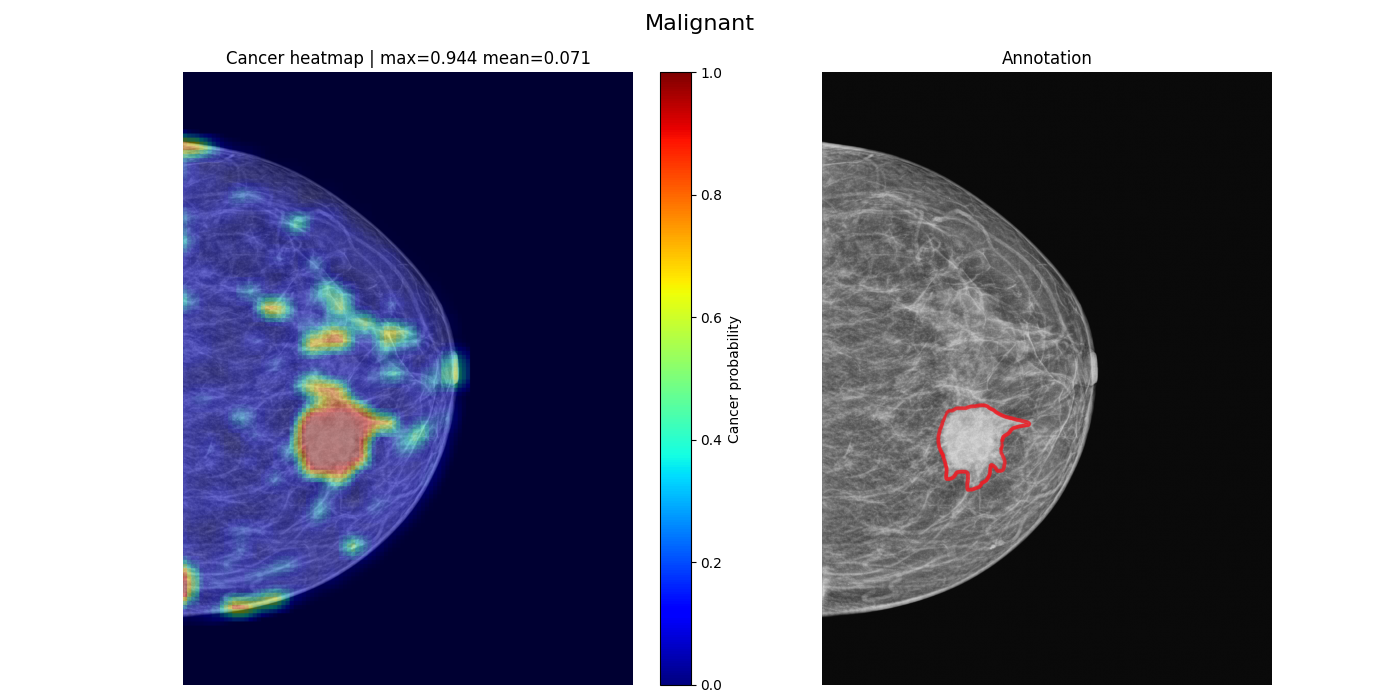
\includegraphics[width=0.50\linewidth]{../results/exp_019/heatmaps/IMG483.tif_heatmap.png}\hfill
    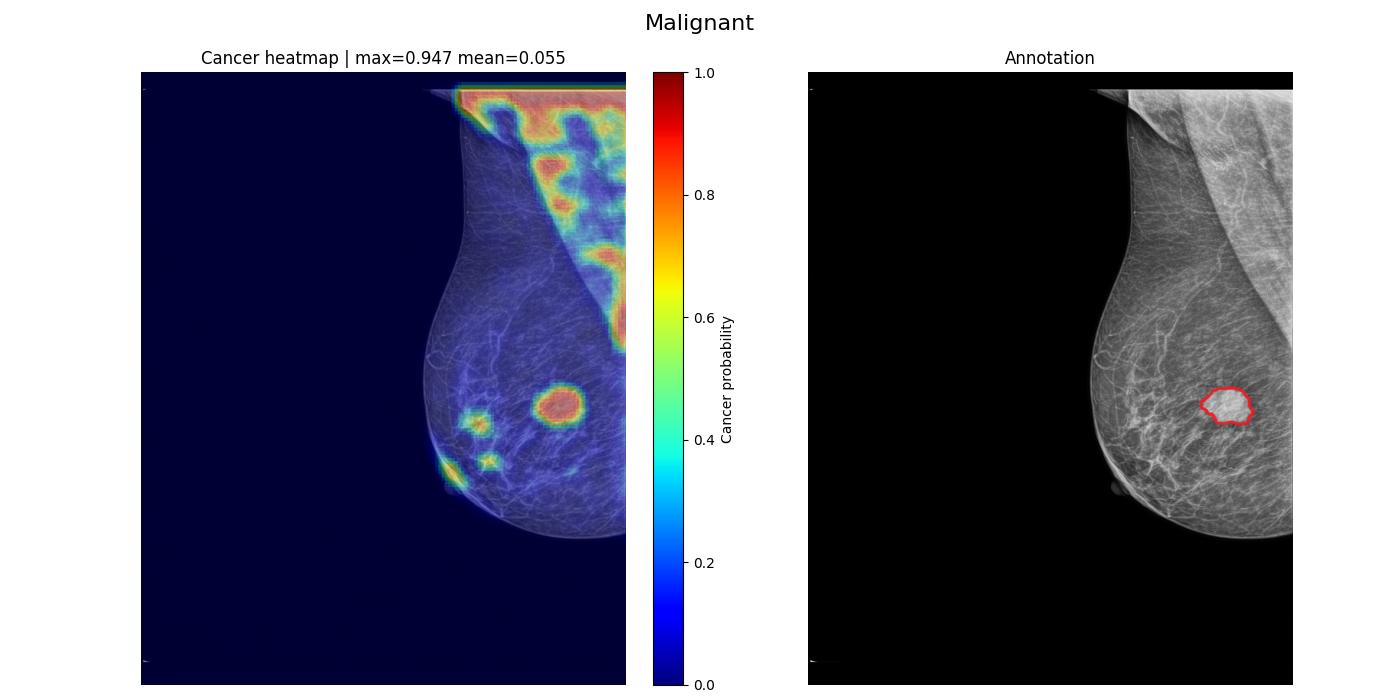
\includegraphics[width=0.50\linewidth]{../results/exp_019/heatmaps/IMG033.tif_heatmap.png}\par\smallskip
    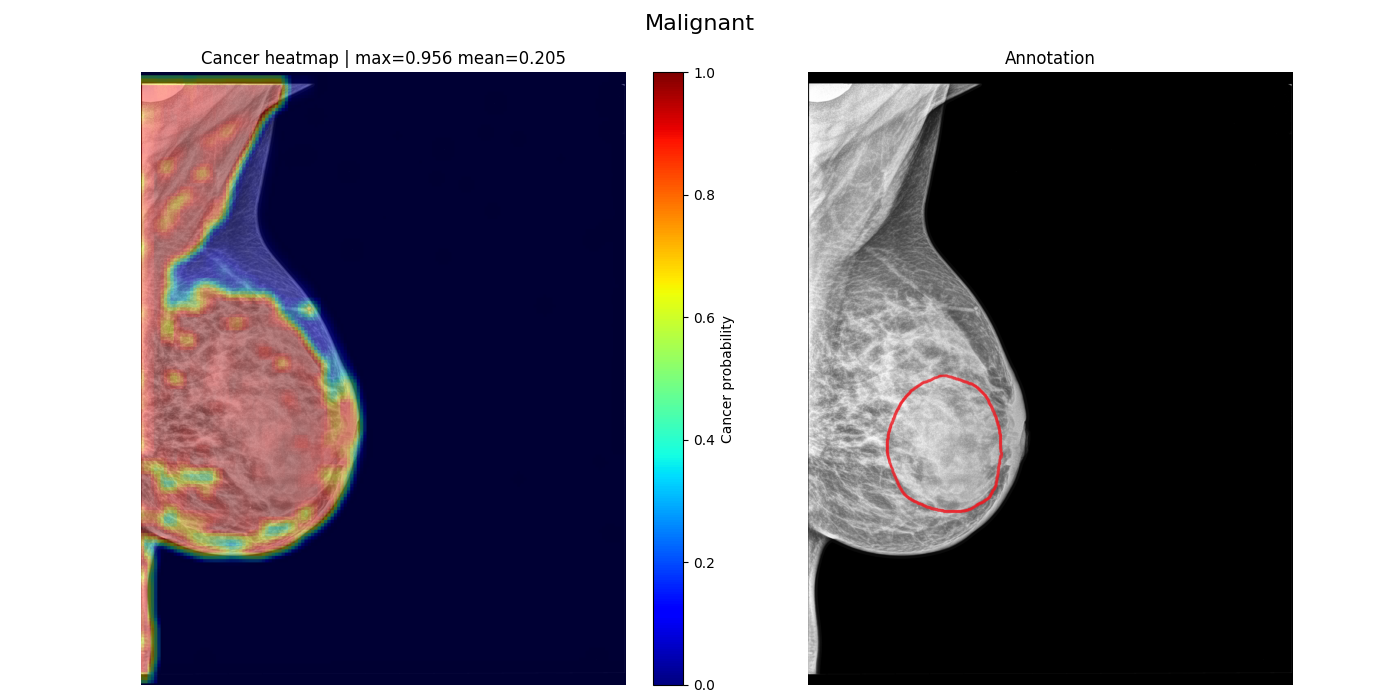
\includegraphics[width=0.50\linewidth]{../results/exp_019/heatmaps/IMG385.tif_heatmap.png}\par\medskip

    % Normal images (separate group)
    \textbf{Normal}\par\medskip
    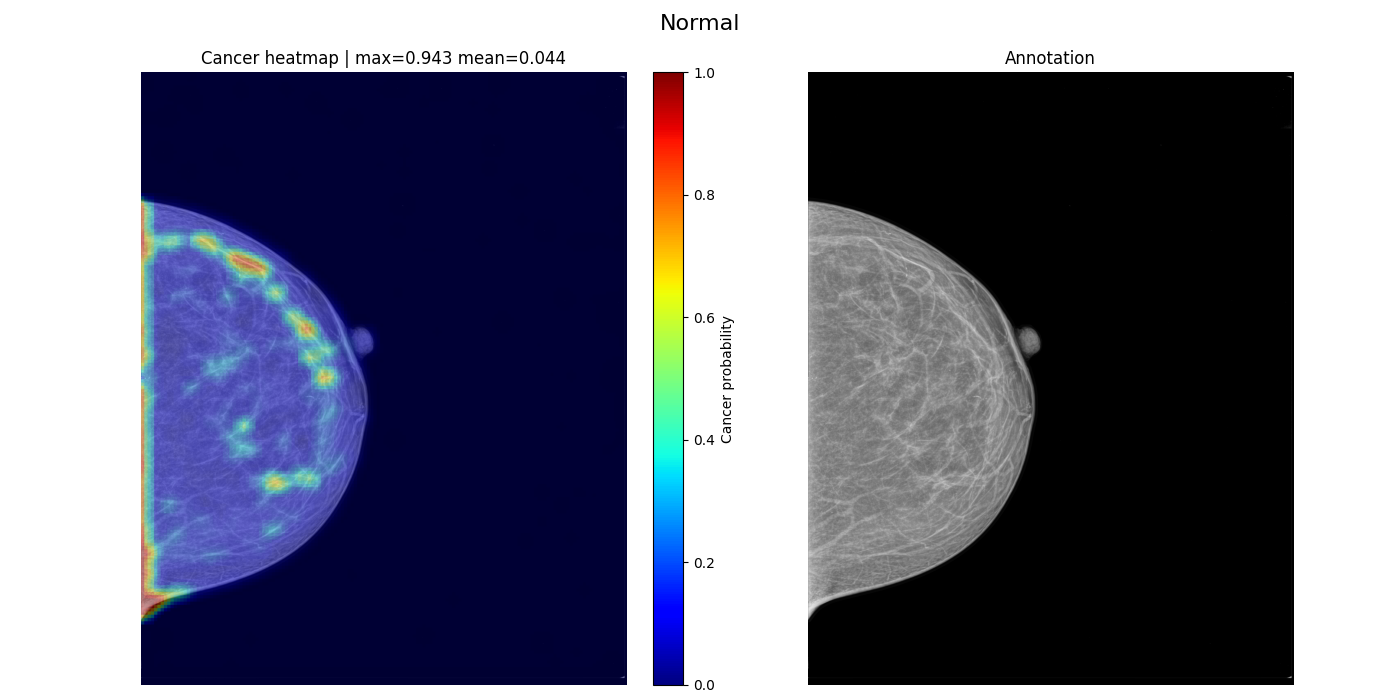
\includegraphics[width=0.50\linewidth]{../results/exp_019/heatmaps/IMG263.tif_heatmap.png}\hfill
    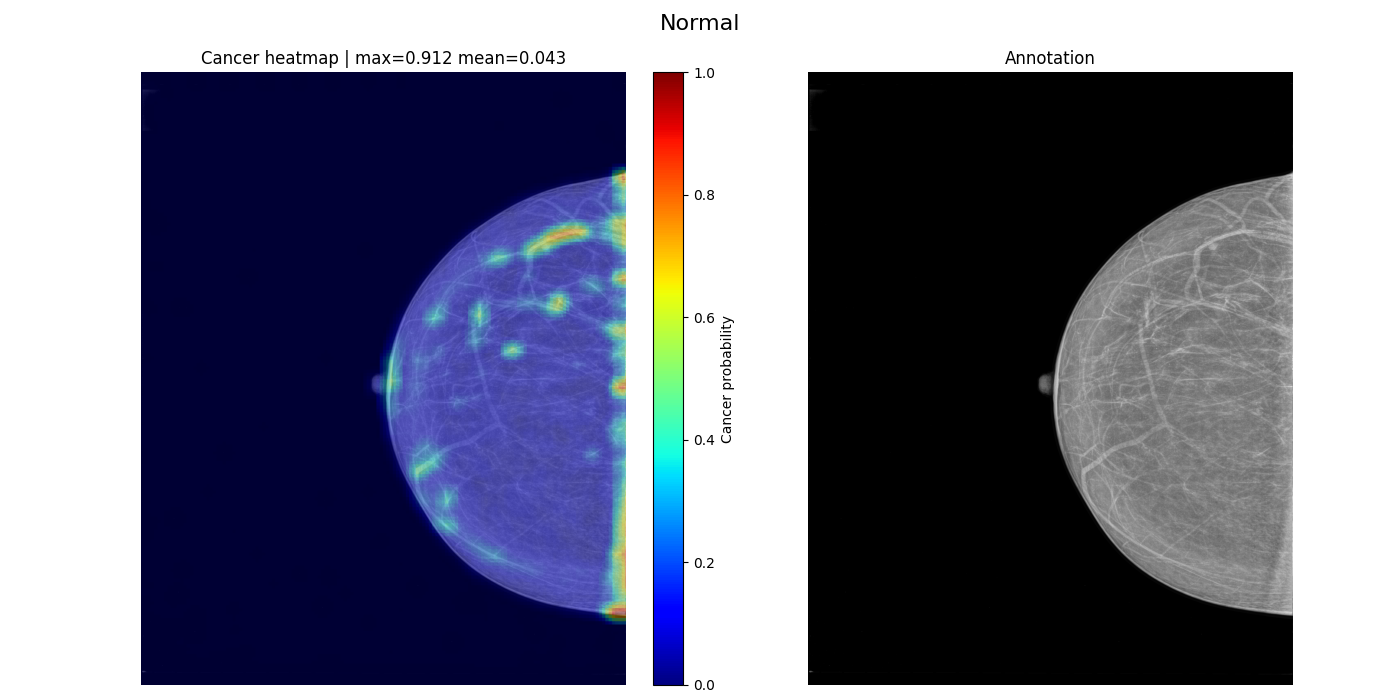
\includegraphics[width=0.50\linewidth]{../results/exp_019/heatmaps/IMG368.tif_heatmap.png}
    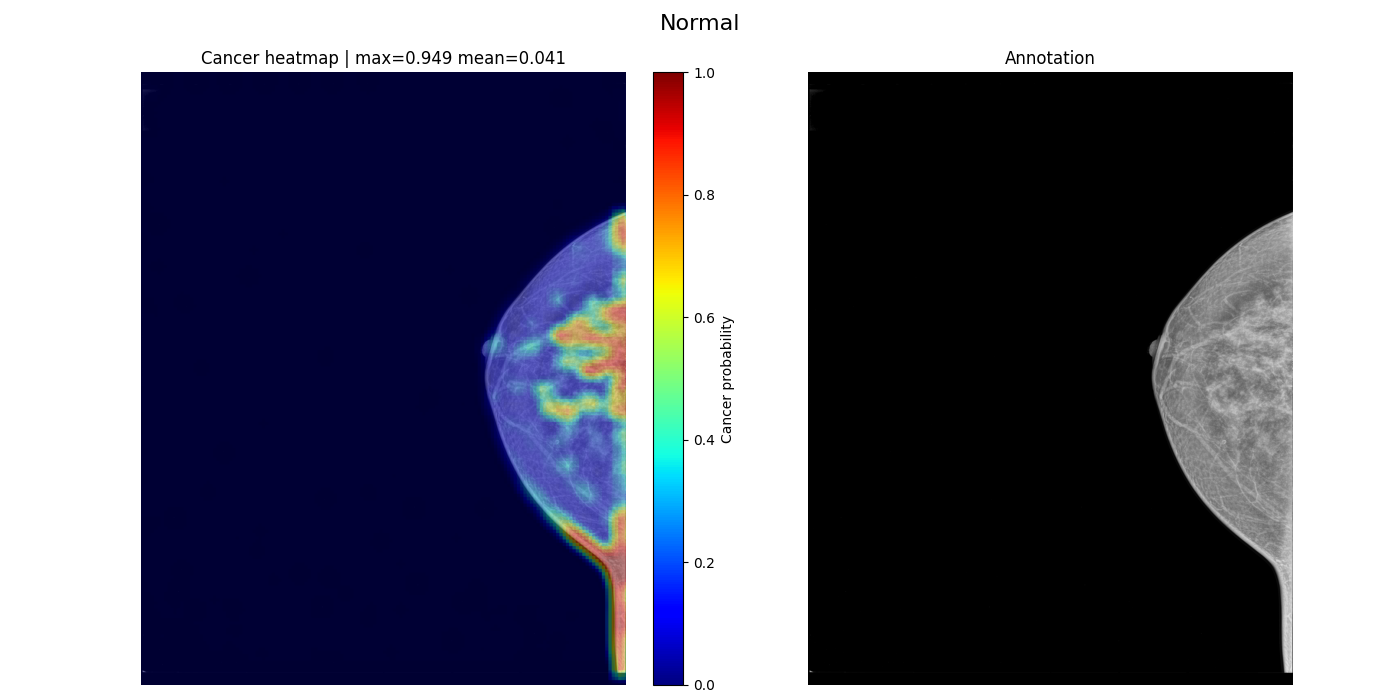
\includegraphics[width=0.50\linewidth]{../results/exp_019/heatmaps/IMG351.tif_heatmap.png}

    \caption{Selected heatmaps for 5 kernel model.}
    \label{fig:exp019_heatmaps}
\end{figure}

\pagebreak

A subset of the images which look like malignant but are considered healthy in the dataset:
\begin{figure}[H]
    \centering
    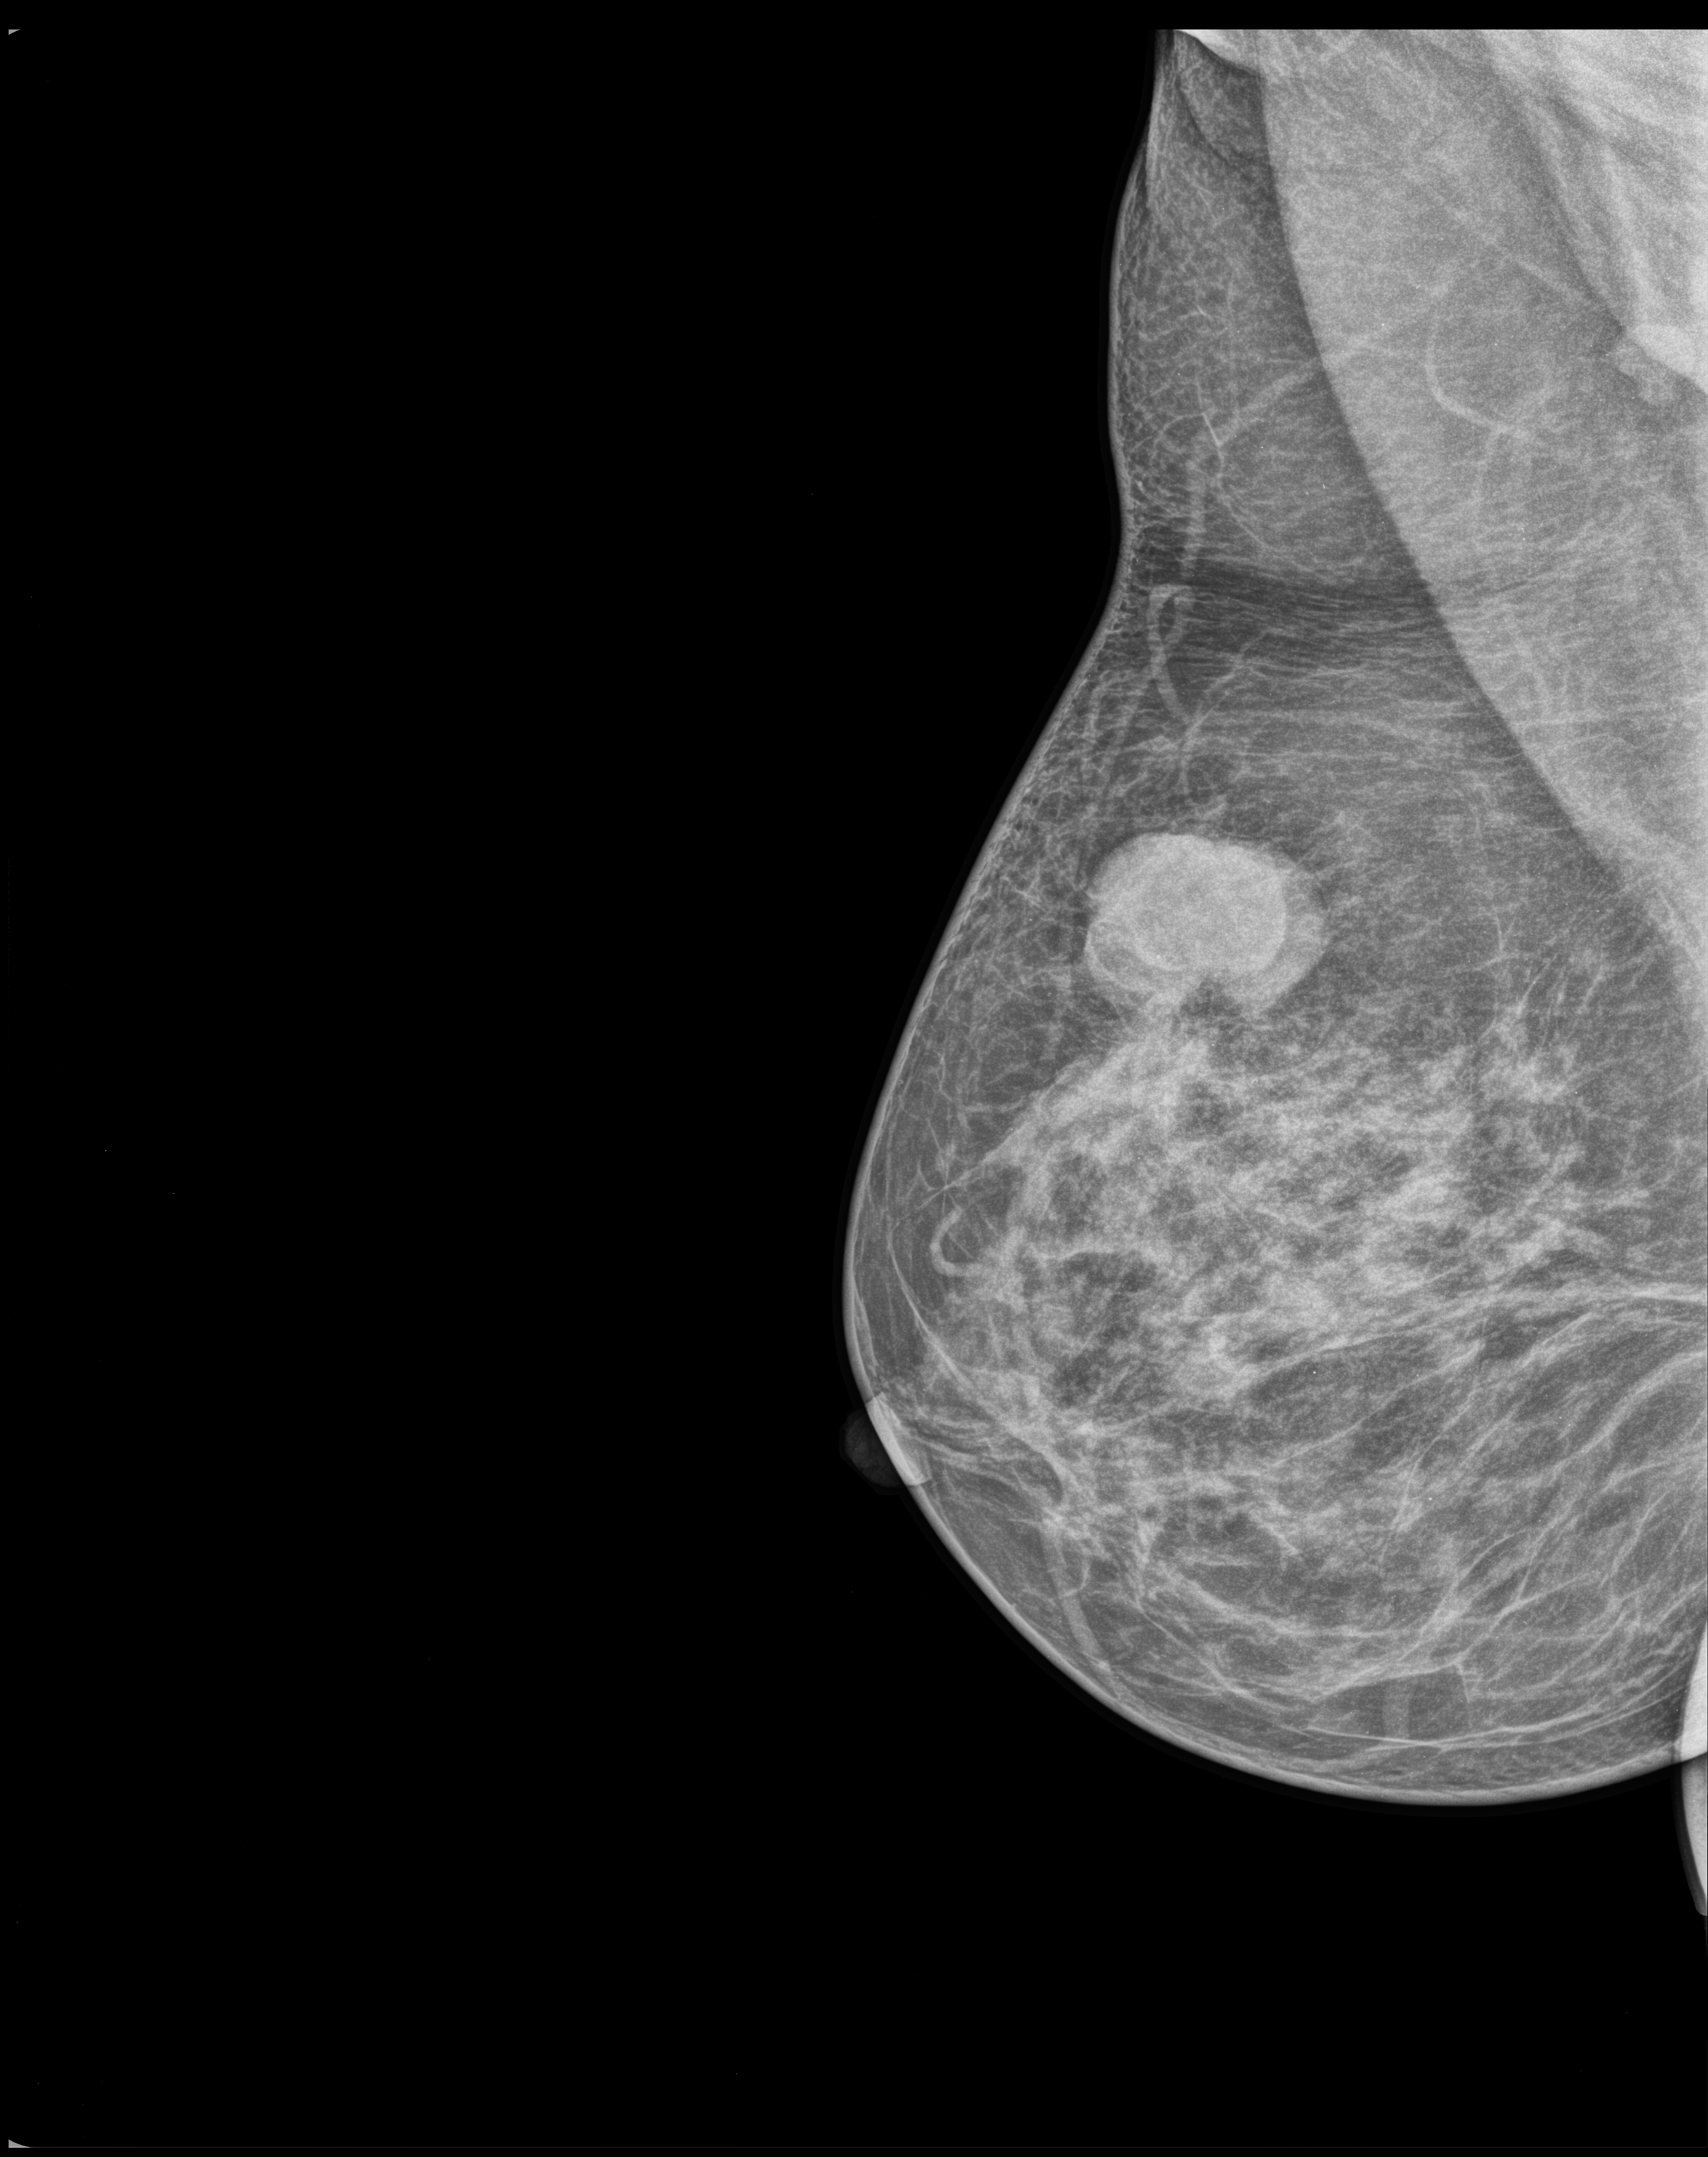
\includegraphics[width=0.48\linewidth]{figures/normal/IMG086.png}\hfill
    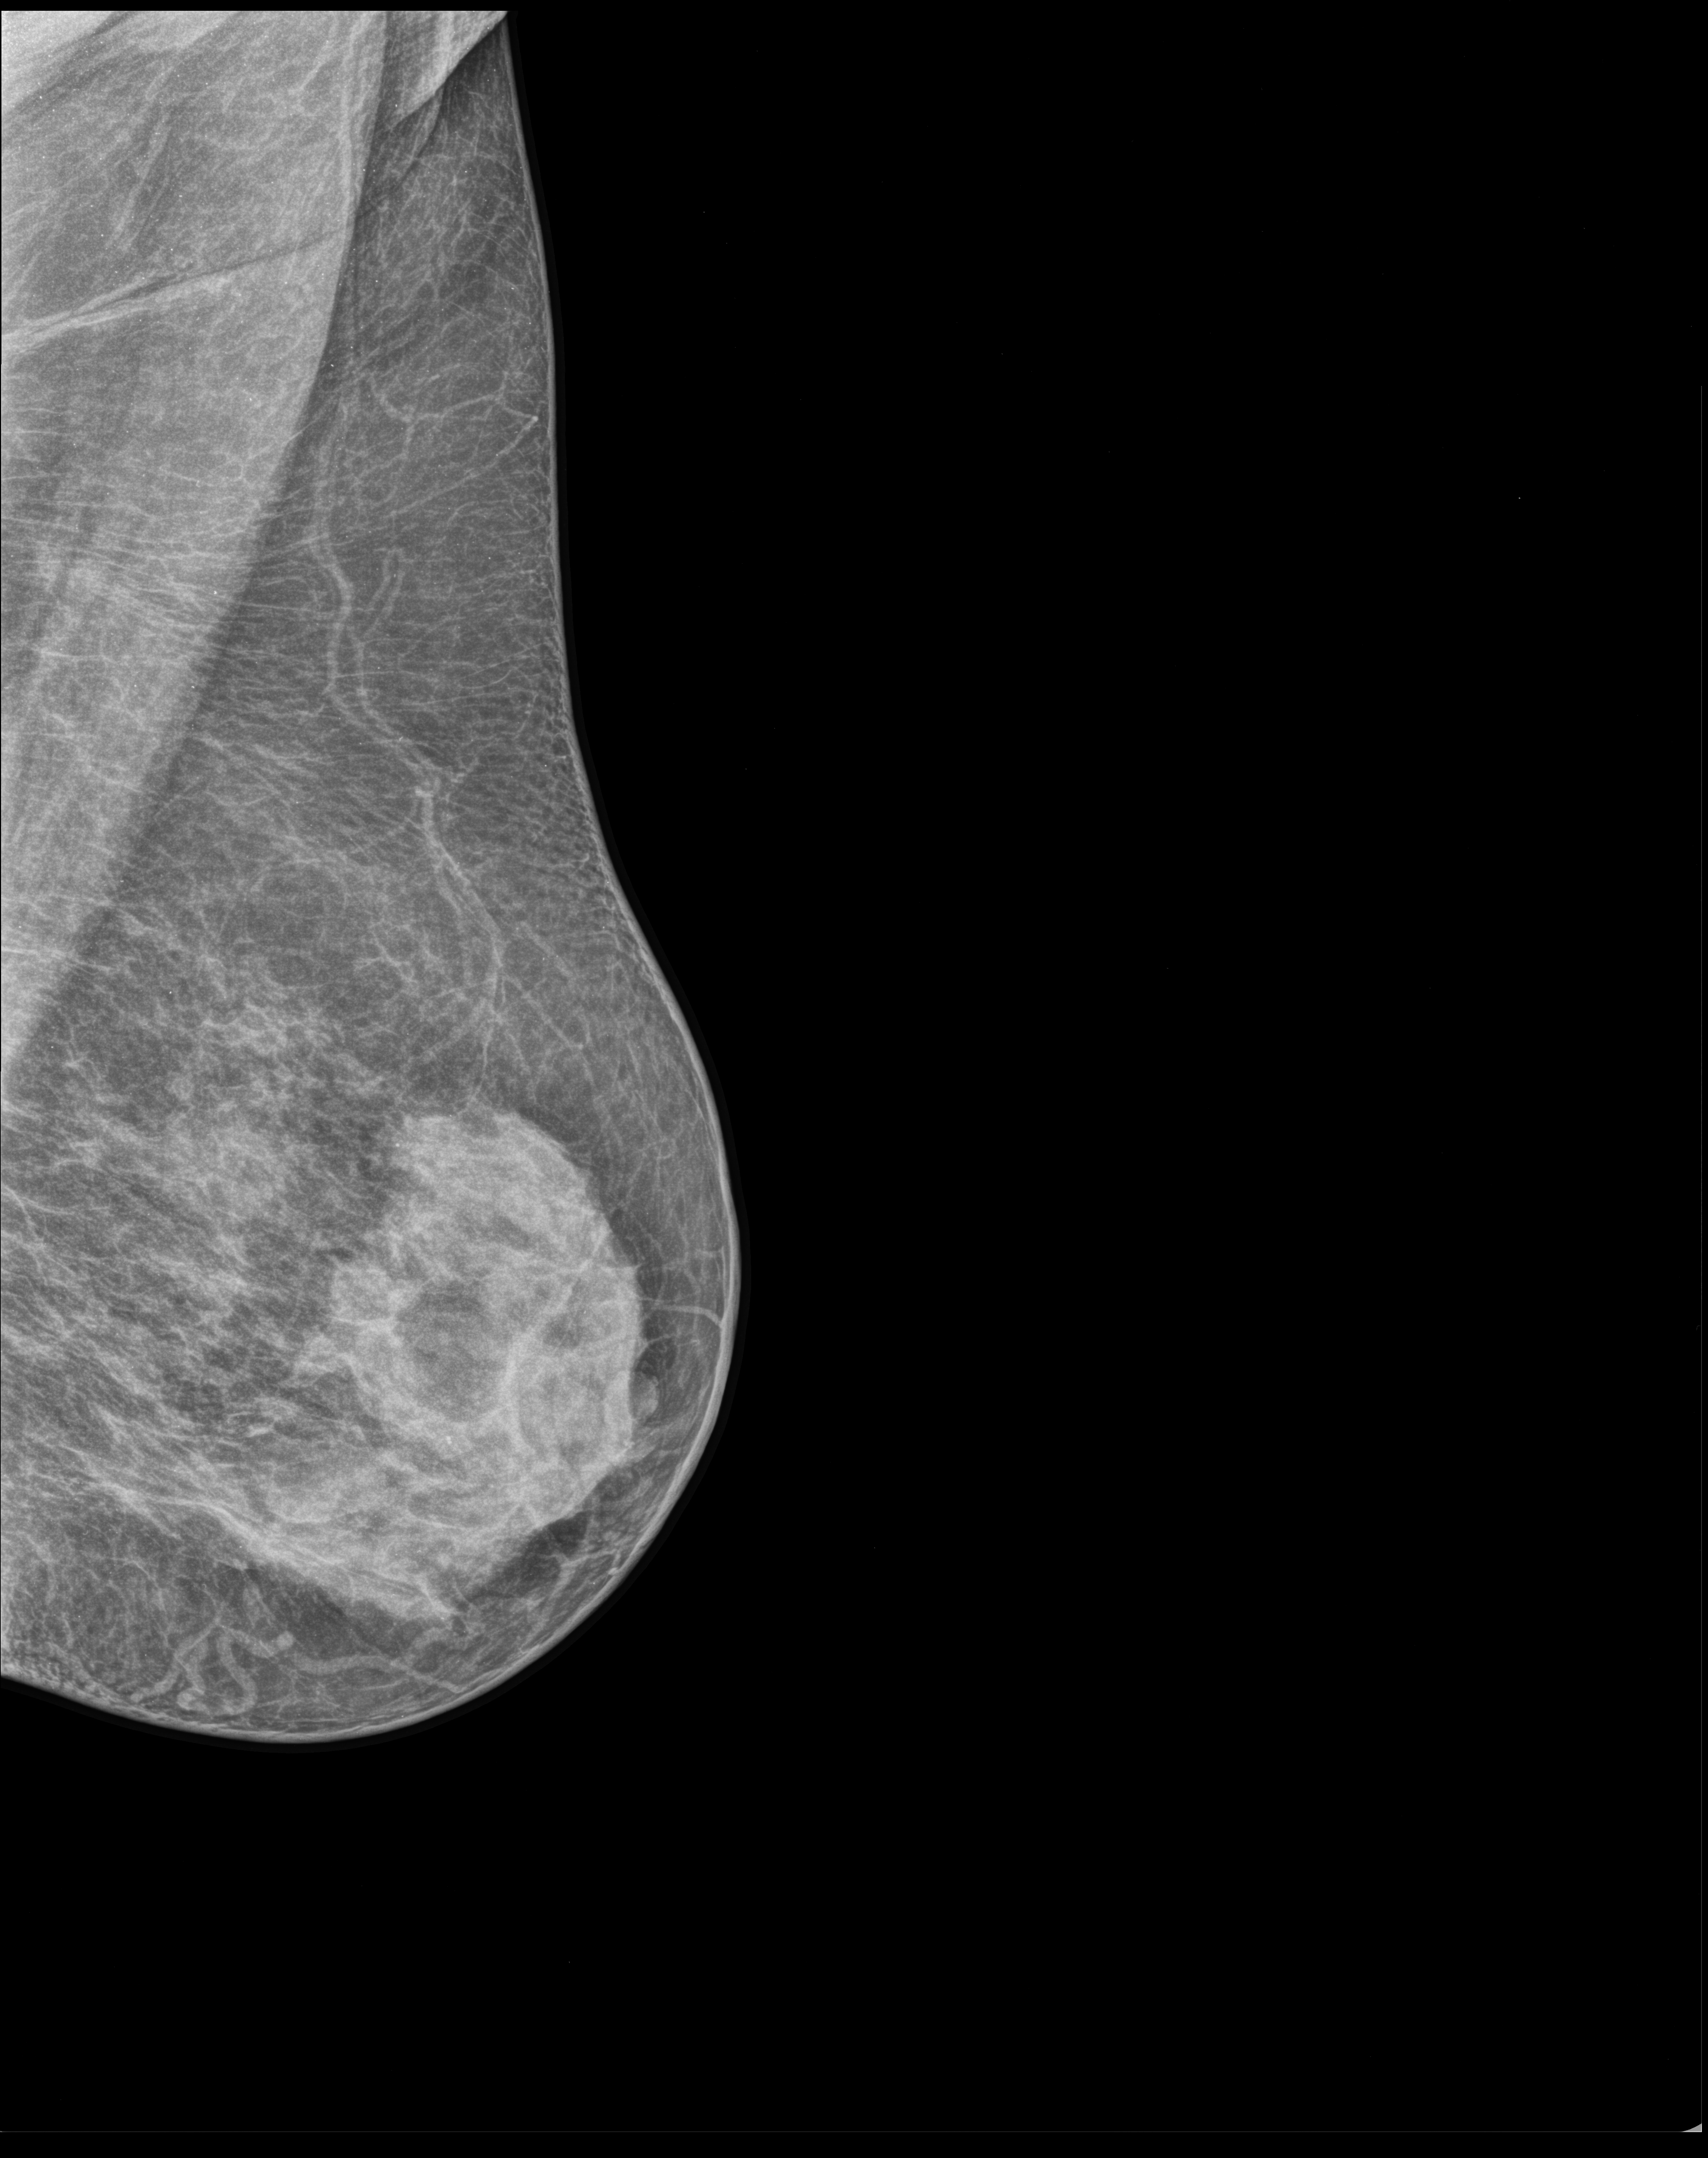
\includegraphics[width=0.48\linewidth]{figures/normal/IMG187.png}\par\smallskip
    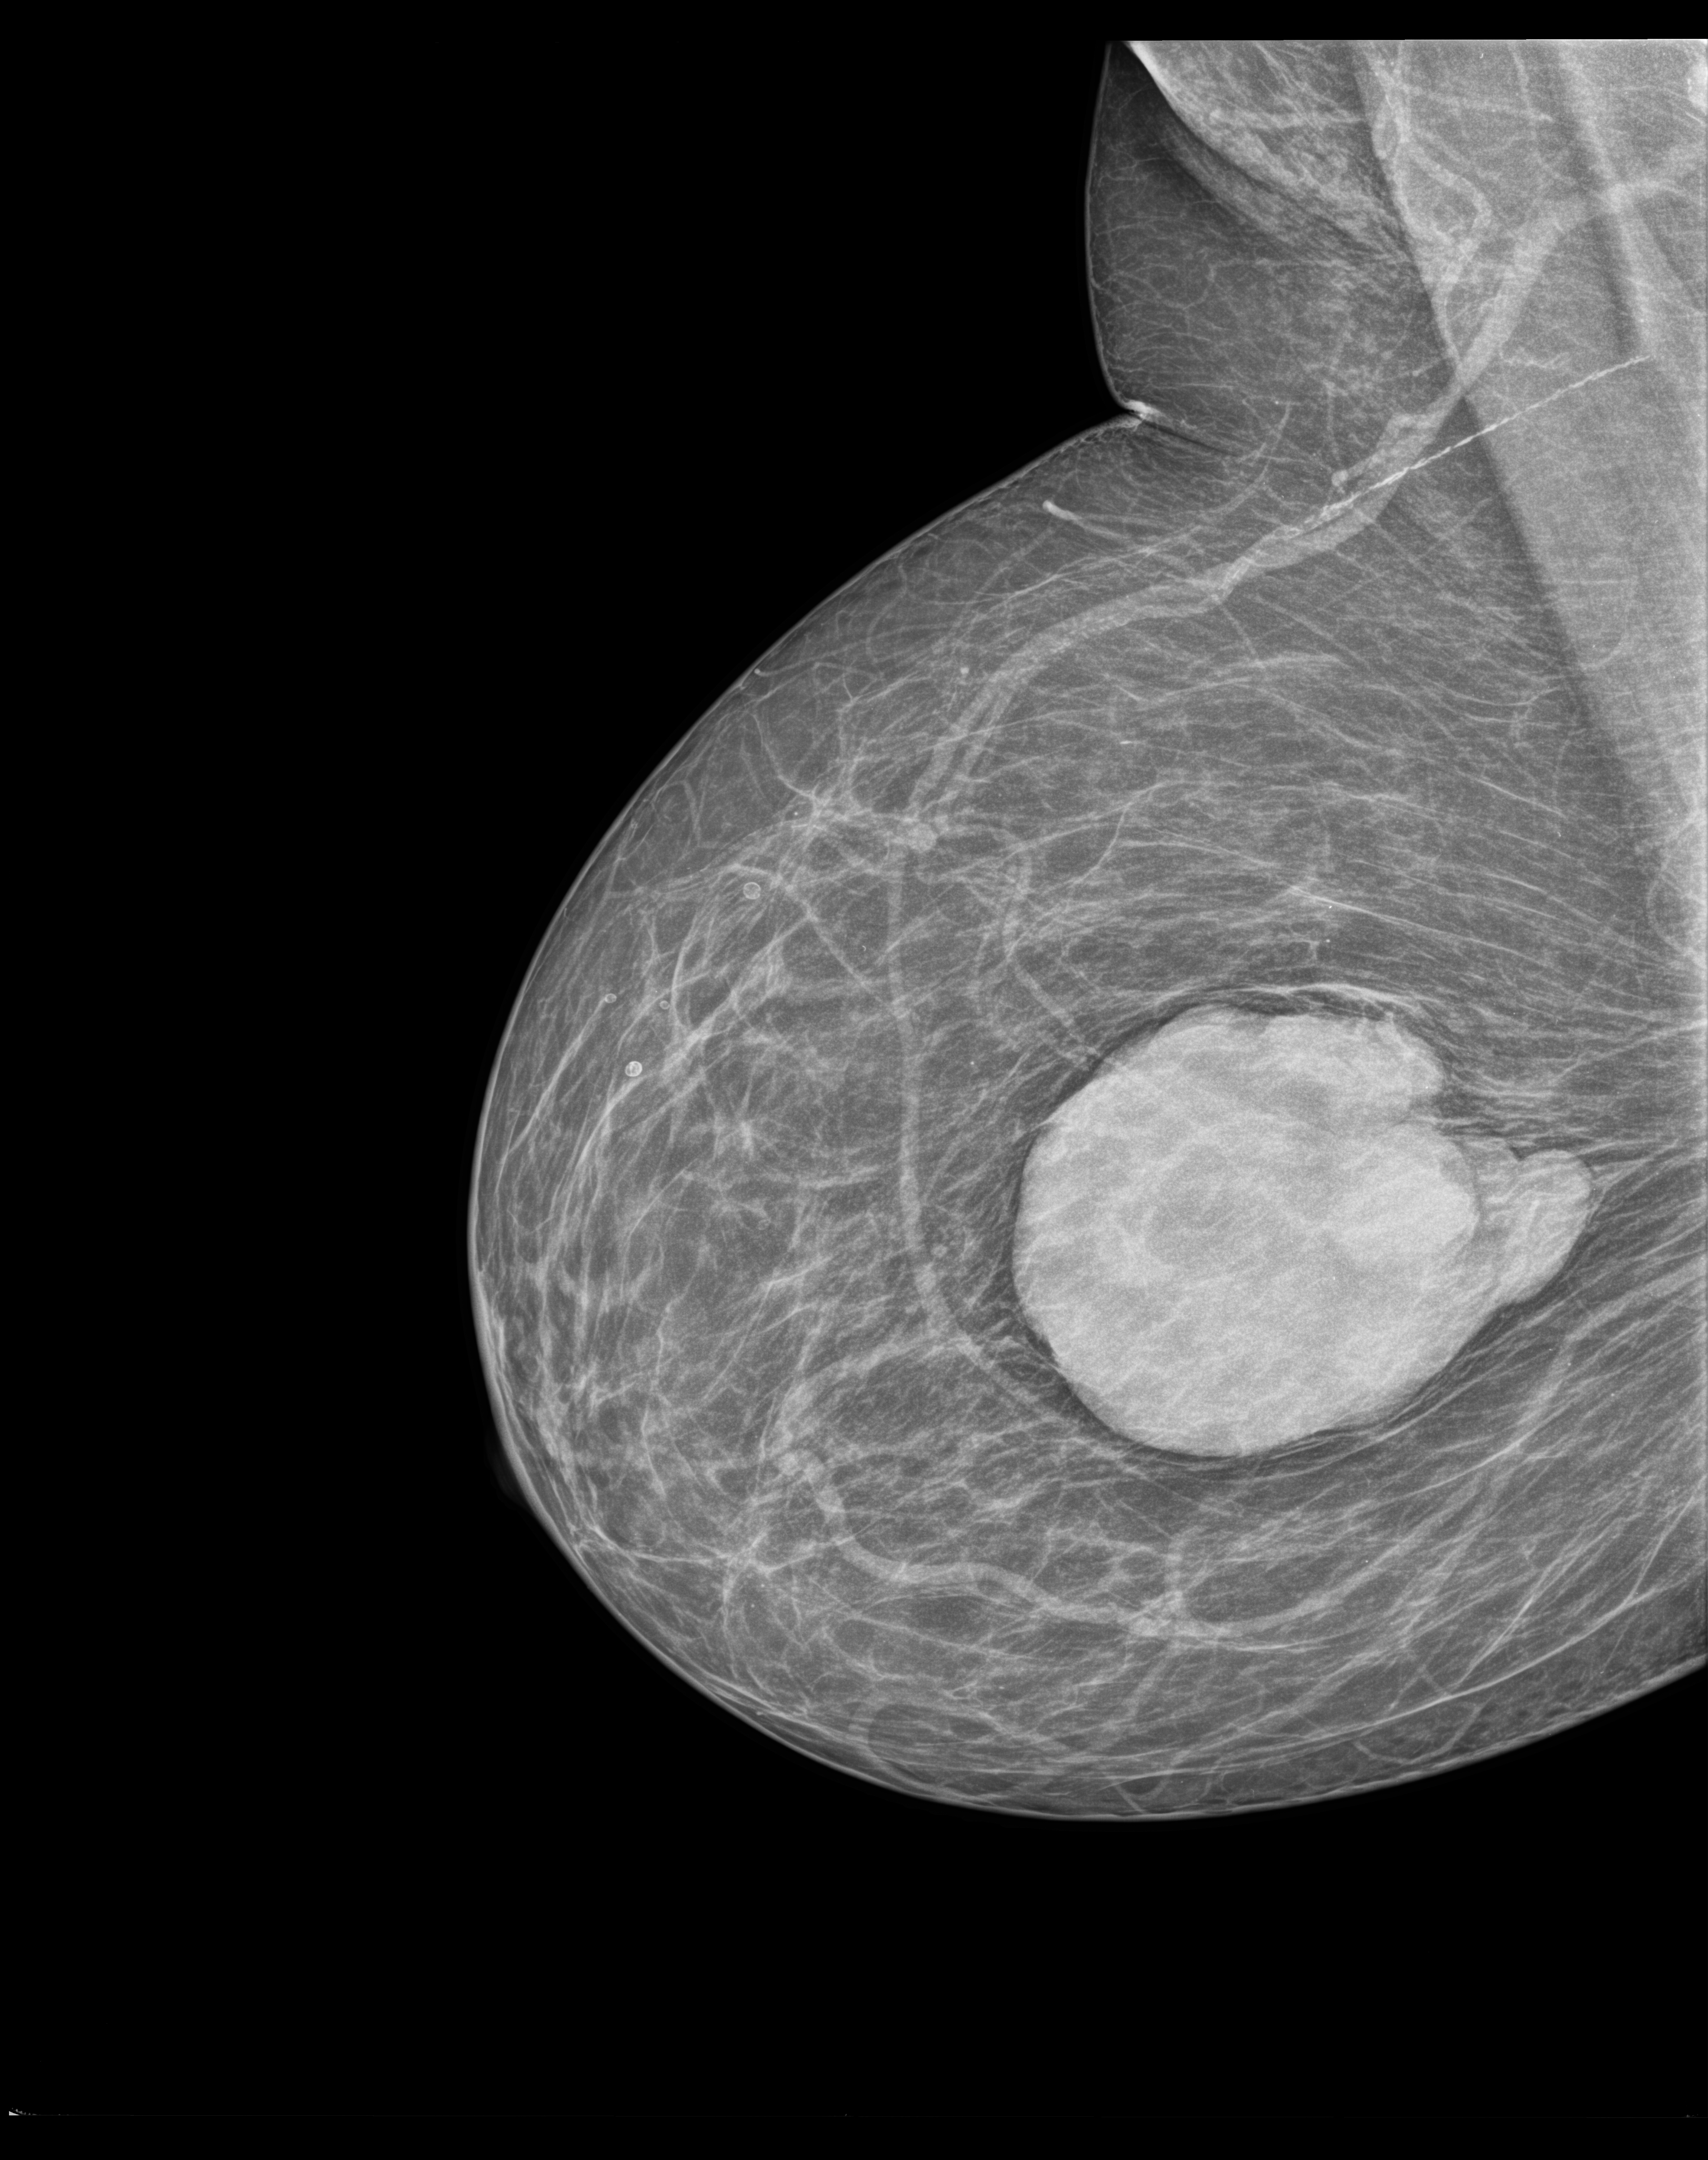
\includegraphics[width=0.48\linewidth]{figures/normal/IMG440.png}\hfill
    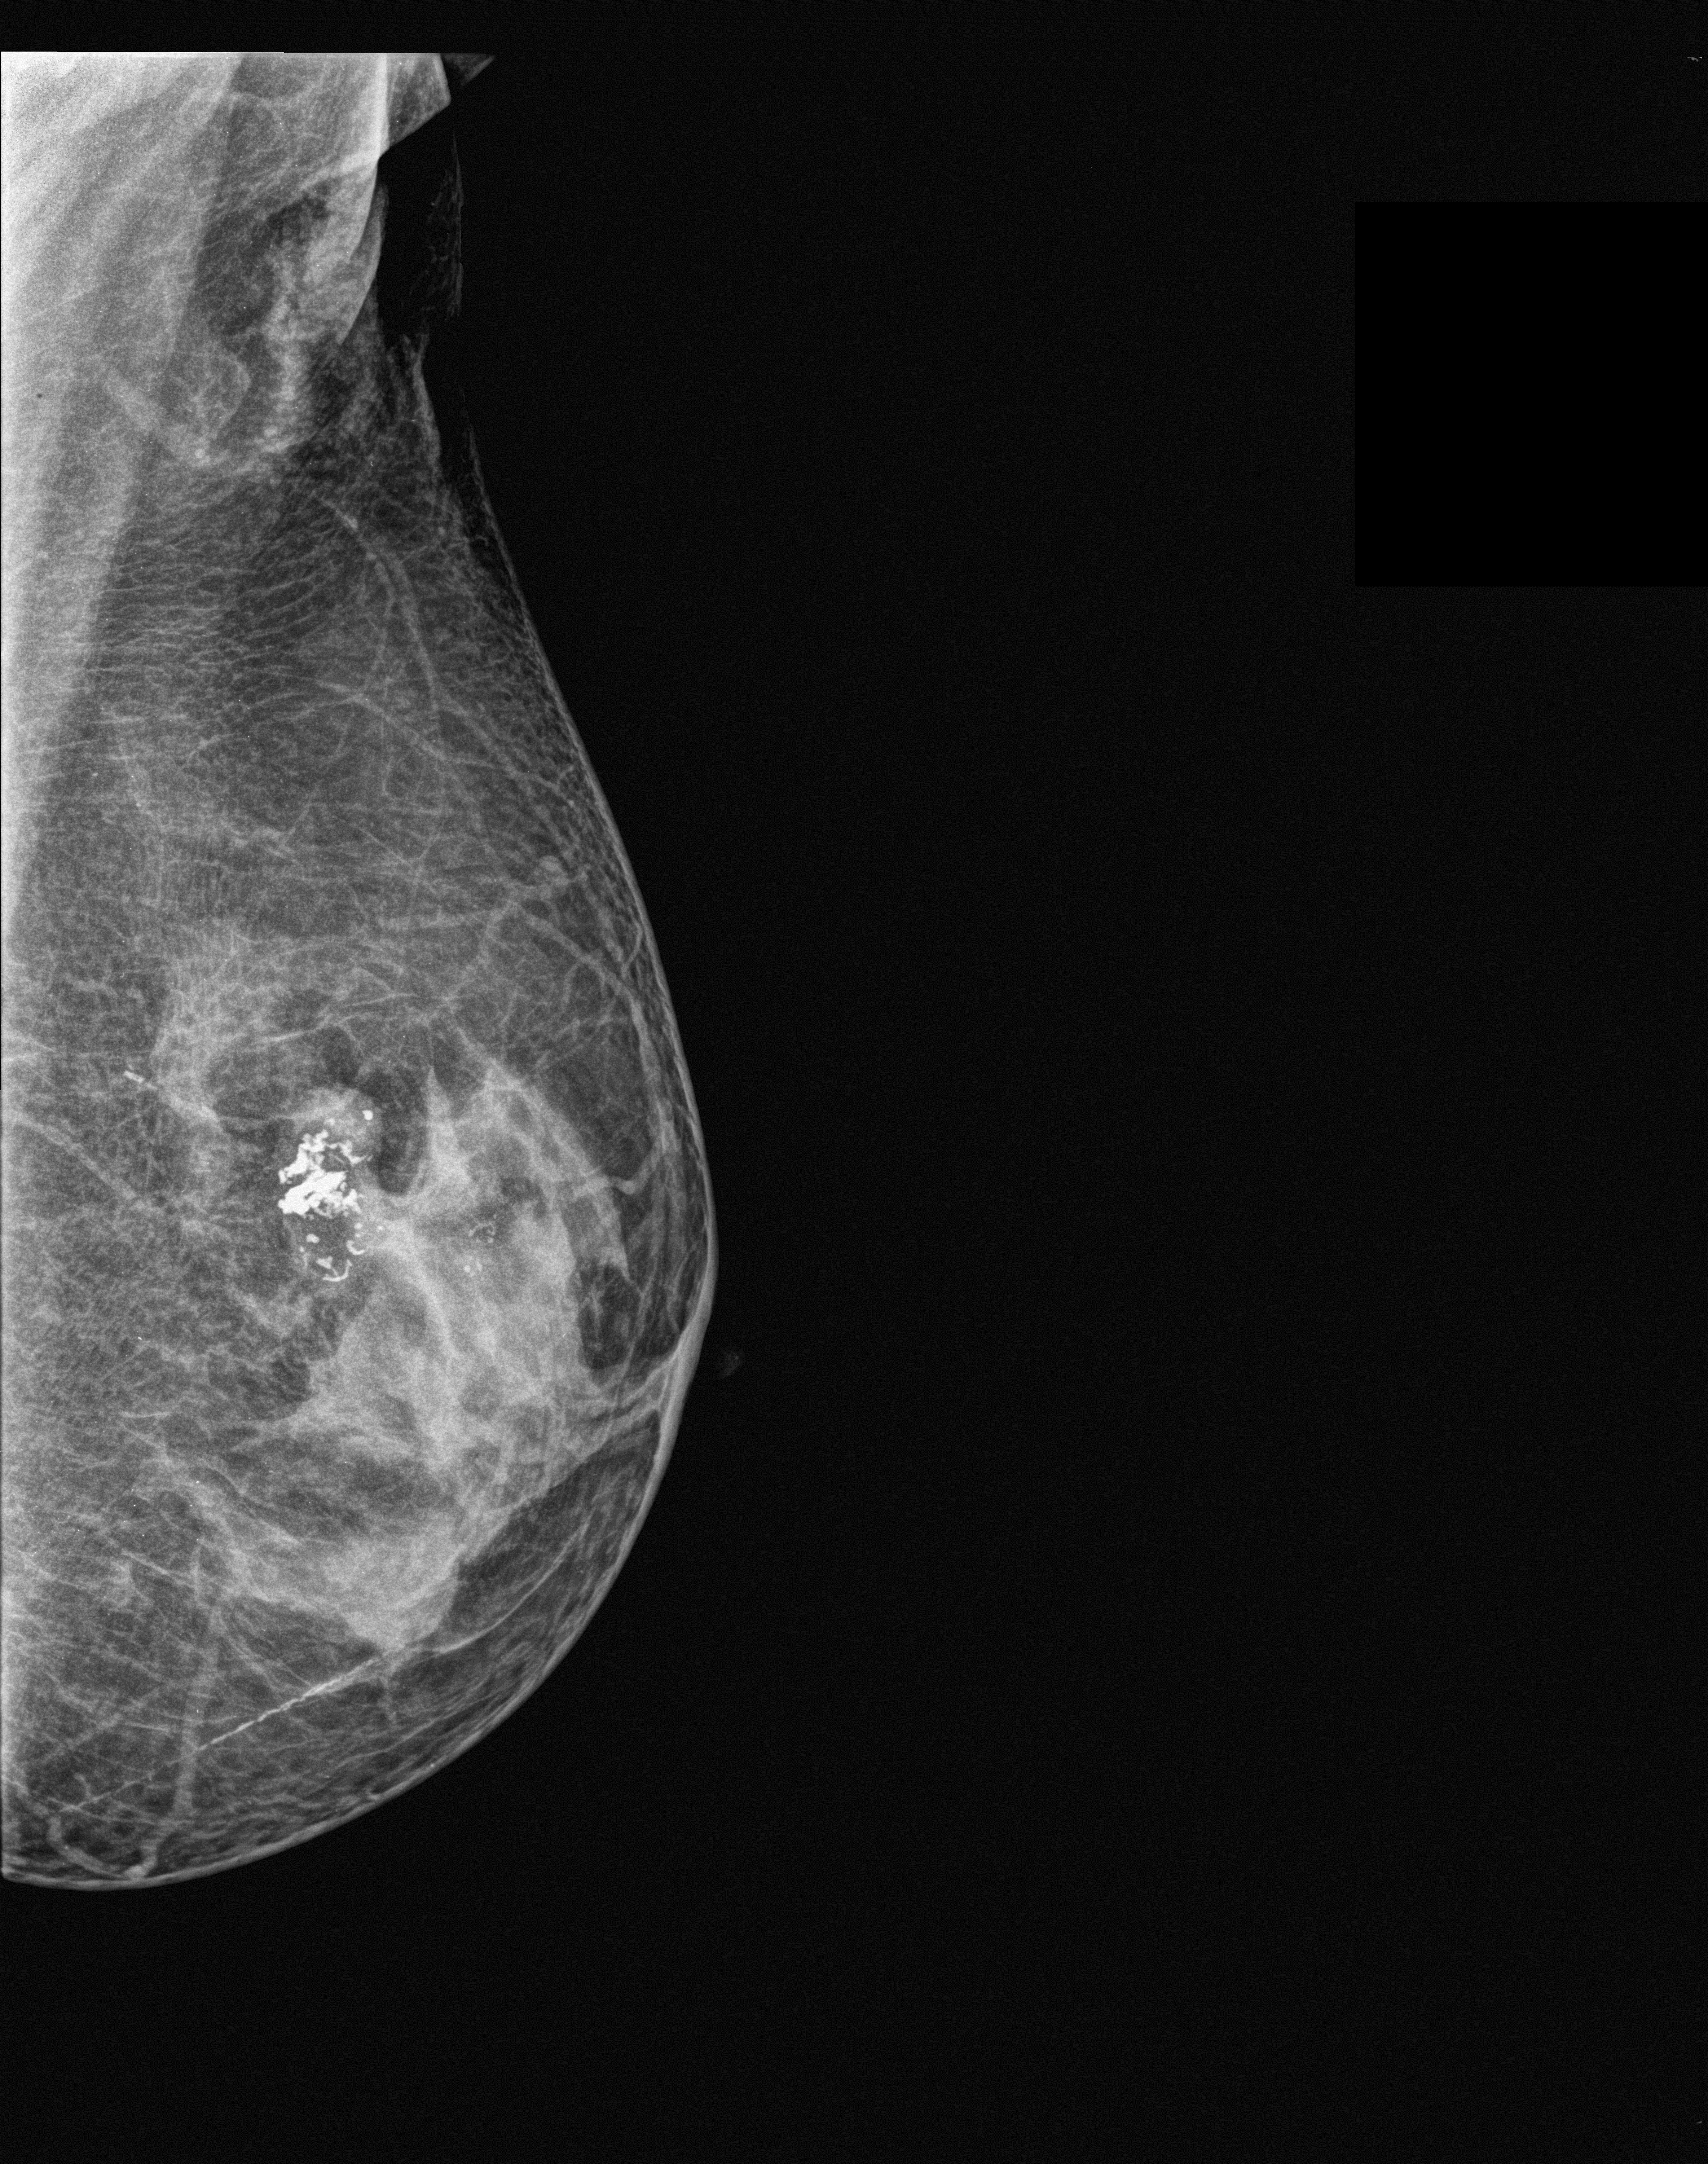
\includegraphics[width=0.48\linewidth]{figures/normal/IMG459.png}
    \caption{Normal-labeled images with malignant-like appearance.}
    \label{fig:normal_malignant_like}
\end{figure}

\end{document}
